\section{Architecture Details}
\label{app:params}

Per temporal layer $12d^2 + 13d$ parameters (four projections, two LayerNorms, feed-forward $4d$); stem $897d$; each residual block $4d^2 + 4d$; positions $128d$; output norm $2d$; a readout of size $V$ has $dV + V$. The v4 depth decoder: context projection $1{,}088 \times 512$, prior embeddings $16{,}384 \times 512 + 6 \times 1{,}024 \times 512$, depth positions $8 \times 512$, two layers of $12 \cdot 512^2 + 13 \cdot 512$, a norm, and seven heads of $512 \times 1{,}024 + 1{,}024$. Table~\ref{tab:params} evaluates these identities for the three widths; the totals are the parameter counts of the released weights, and the eight transformer layers hold 62\% of v1 and 67\% of v4.

\begin{table}[tb]
\centering\small
\caption{Parameter breakdown of the released encoders.}
\label{tab:params}
\adjustbox{max width=\columnwidth}{\begin{tabular}{lrrr}
\toprule
Component & v1 ($d{=}512$) & v2, v3 ($d{=}1{,}088$) & v4 \\
\midrule
stem & 459,264 & 975,936 & 975,936 \\
residual blocks & 3,151,872 & 14,217,984 & 14,217,984 \\
positions & 65,536 & 139,264 & 139,264 \\
transformer & 25,219,072 & 113,752,576 & 113,752,576 \\
output norm & 1,024 & 2,176 & 2,176 \\
readouts & 12,082,176 & 25,648,128 & 17,842,176 \\
depth decoder & 0 & 0 & 22,078,464 \\
\midrule
total & 40,978,944 & 154,736,064 & 169,008,576 \\
\bottomrule
\end{tabular}}
\end{table}

\section{Additional Experiments}
\label{app:extra}

\paragraph{Benchmarks.} Figure~\ref{fig:bench} shows the two measurements that decided the kernel choices of Sec.~\ref{sec:encoder}, taken on an NVIDIA GeForce RTX 3090 (sm\_86, 23.6 GiB), torch 2.14 on CUDA 13, bfloat16 autocast, tf32 enabled, with latency as the median device time over repetitions. Top: at the temporal stack's shape the fused kernel is 3.6$\times$ faster forward and 2.8$\times$ faster backward, and at the depth decoder's shape it is 2.9x and 3.8$\times$ slower, because a sequence of length 8 is below the tile size of the fused kernels and their set-up dominates. Bottom: assembling the pooling operator for a batch on the host costs 152.9 ms as dense matrices and 8.5 ms as segment indices at batch 64, and 19.8 ms against 1.8 ms at batch 16.

\begin{figure}[tb]
  \centering
  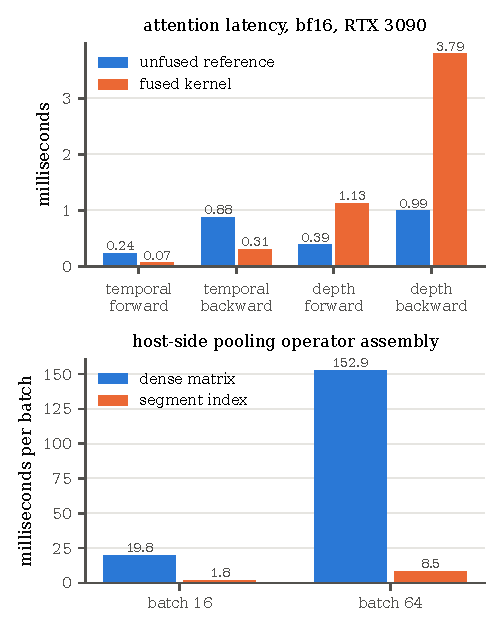
\includegraphics[width=\columnwidth]{figures/benchmarks.pdf}
  \caption{Top: attention latency at the two shapes the model runs; the fused kernel wins on the temporal stack and loses on the depth decoder. Bottom: host-side assembly of the pooling operator per batch, dense matrix against segment index.}
  \label{fig:bench}
\end{figure}

\paragraph{Held-out metrics over training.} Figure~\ref{fig:checkpoints} scores all 36 checkpoints of each run on the full held-out split. Semantic top-1 (first panel) climbs steeply for 4,000 steps and then slowly; the three wide models track one another and the 41M model runs two points below them throughout. Acoustic top-1 (second panel) shows the same ordering for the free-running curves, while the dashed teacher-forced v4 curve keeps rising to 18\% and opens the exposure gap steadily from the first checkpoint on. The held-out loss of the independent-head models (third panel) is directly comparable across v1 to v3; the v4 loss (fourth panel) is conditional on the true earlier codes and is drawn on its own axis. All curves are still improving at 17,660 steps.

\begin{figure}[tb]
  \centering
  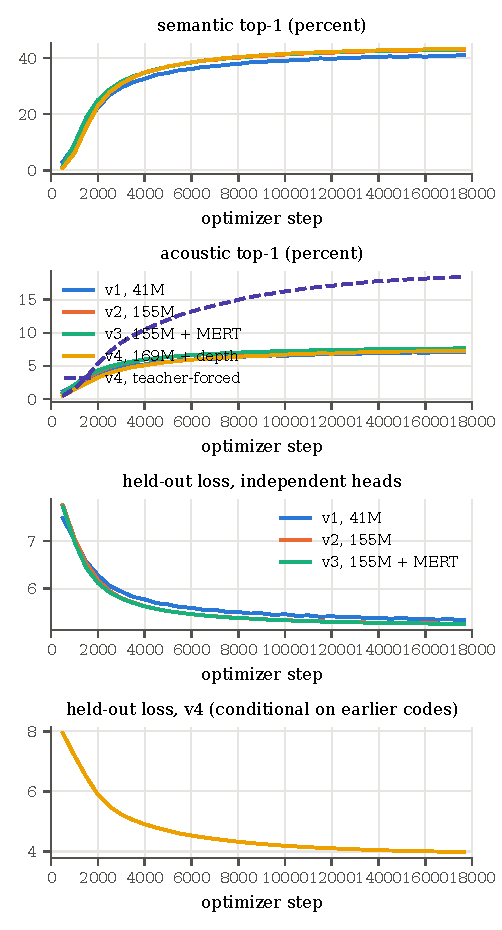
\includegraphics[width=\columnwidth]{figures/checkpoints.pdf}
  \caption{Held-out metrics over the checkpoints of every run: semantic top-1, acoustic top-1, held-out loss of the independent-head models, and the v4 loss, which is conditional on the true earlier codes and has its own panel.}
  \label{fig:checkpoints}
\end{figure}

\paragraph{Training dynamics.} Figure~\ref{fig:history} shows the training loss (top) as a running mean over 15 logged steps and the learning rate of the width-scaled parameter group relative to its peak (bottom). The loss curves order as the held-out curves do, with v4 lower because its objective is conditional. The learning-rate panel makes the schedule difference between the runs explicit: v1 follows a cosine of half period 500 that returns to its peak every 1,000 steps, whereas v2 to v4 warm up for 500 steps and decay linearly to $10^{-7}$; the v1 loss shows no visible ripple at the reheating points.

\begin{figure}[tb]
  \centering
  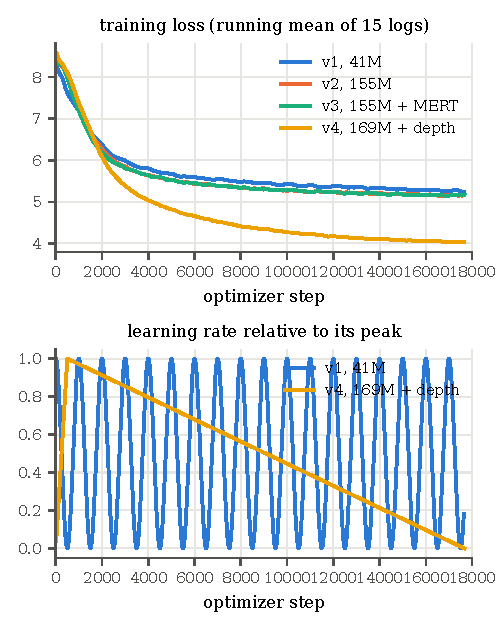
\includegraphics[width=\columnwidth]{figures/history.pdf}
  \caption{Training loss (top) and learning rate of the width-scaled parameter group relative to its peak (bottom): the v1 cosine schedule reheats every 1,000 steps, v2 to v4 warm up for 500 steps and decay linearly.}
  \label{fig:history}
\end{figure}

\paragraph{Packaged checkpoints.} v2 to v4 ship their final checkpoint at step 17,660; their held-out metrics are the published rows of Tab.~\ref{tab:reproduced}. v1 ships step 17,500 (loss 5.3379, semantic top-1 41.03\%, acoustic top-1 7.17\%), the best of its run by loss and top-1; its final checkpoint at step 17,640 is 0.003 worse in loss, a consequence of the cosine schedule ending mid-cycle. The v1 replay cosine in Tab.~\ref{tab:replay} was measured on the final checkpoint and the packaged one differs from it by 140 optimizer steps.

\paragraph{Reproducibility.} Table~\ref{tab:reproduced} places each published held-out row beside the row obtained by re-evaluating the released weights on one RTX 3090, from latents recomputed from the held-out audio. The loader yields the same 135 held-out records, 130 exact, and 2,768 windows. Every published row is reproduced within 0.003 in loss and 0.001 in accuracy under bfloat16 autocast, the teacher-forced column included, and the full float32 row for v4 moves by a further 0.001; the residual differences are float reassociation across kernels and ranks.

\begin{table}[tb]
\centering
\small
\caption{Published rows against our implementation on the same held-out split.}
\label{tab:reproduced}
\adjustbox{max width=\columnwidth}{
\begin{tabular}{lrrrrrrr}
\toprule
Model & Source & Loss & Sem. top-1 & Sem. top-5 & Ac. top-1 & Ac. top-5 & TF ac. top-1 \\
\midrule
v1, 41M & published, bf16, 4 ranks & 5.3379 & 41.03 & 7.17 &  \\
v1, 41M & this repository, bf16, 1 GPU & 5.3353 & 41.08 & 7.18 &  \\
v2, 155M & published, bf16, 4 ranks & 5.2644 & 42.86 & 7.62 &  \\
v2, 155M & this repository, bf16, 1 GPU & 5.2644 & 42.86 & 7.62 &  \\
v3, 155M + MERT & published, bf16, 4 ranks & 5.2599 & 43.03 & 7.66 &  \\
v3, 155M + MERT & this repository, bf16, 1 GPU & 5.2574 & 43.07 & 7.67 &  \\
v4, 169M + depth & published, bf16, 4 ranks & 3.9874 & 43.17 & 7.29 & 18.42 \\
v4, 169M + depth & this repository, bf16, 1 GPU & 3.9860 & 43.24 & 7.30 & 18.44 \\
v4, 169M + depth & this repository, fp32, 1 GPU & 3.9858 & 43.26 & 7.30 & 18.44 \\
\bottomrule
\end{tabular}
}
\end{table}


\paragraph{Provenance.} Table~\ref{tab:provenance} records where each released weight file came from: the training run (a repository under SimpleTuner/open-rvq-encoder-minimax-music3) and its revision, the checkpoint that was packaged, and the leading digits of the weight file's checksum, together with the dataset revision used for every number in this paper. Replay evaluation used the official components at revision fbdf52fb, and the community checkpoint is best.pt from commit d19efe9f of minimaxmusic.cpp~\cite{serveurperso2026encoder}.

\begin{table}[tb]
\centering
\small
\caption{Release provenance.}
\label{tab:provenance}
\adjustbox{max width=\columnwidth}{
\begin{tabular}{lrrrr}
\toprule
Version & Source run & Revision & Checkpoint & Weights sha256 \\
\midrule
v1 & 41m-v1 & e9fa3bba9b5b & checkpoint-17500 & 9683ba0a719fc8f4 \\
v2 & 155m-v2 & f317d72466b9 & final & 47dfffb7a76d9558 \\
v3 & 155m-v3 & 7c525705817d & final & 356e97fea65c486a \\
v4 & 169m-v4 & b9a9165b99d1 & final & e8fa93a7db2e5a09 \\
dataset & minimax-music3-rvq-reverse-distillation & 5029b1e7f1bb & holdout &  \\
\bottomrule
\end{tabular}
}
\end{table}



\section{Hyperparameters}
\label{app:hyper}

Table~\ref{tab:hyper} lists every setting of the four runs; the values are those of the released configurations, and the rows marked with a version apply to that run only.

\begin{table}[H]
\centering\small
\caption{Training and evaluation hyperparameters shared by all runs unless noted.}
\label{tab:hyper}
\adjustbox{max width=\columnwidth}{\begin{tabular}{ll}
\toprule
Setting & Value \\
\midrule
hardware & 4 x NVIDIA L40S, PyTorch DDP \\
precision & bfloat16 autocast, tf32 matmul \\
epochs, optimizer steps & 20, 17,660 (v1: 17,640) \\
batch per rank, global & 16, 64 \\
optimizer & AdamW under $\mu$P, $\beta = (0.9, 0.999)$, $\epsilon = 10^{-8}$ \\
learning rate, weight decay & $3 \times 10^{-4}$, 0.01 \\
schedule, v1 & cosine, half period 500 steps, no warm-up \\
schedule, v2 to v4 & linear warm-up 500 steps, linear decay to $10^{-7}$ \\
gradient norm limit & 1.0 \\
$\mu$P base width, multiplier & 128; 4 (v1), 8.5 (v2 to v4) \\
attention scale & $8 / d_h$, $d_h = 64$ \\
dropout & 0.1 \\
window, stride & 128 frames, random crop (train), 128 (validation) \\
KL weight, temperature, top-$k$ & 0.25, 1.0, 50 \\
MERT term, v3 only & layer 4 to teacher layer 9, weight 0.5 to 0.7 $T$, zero by 0.9 $T$ \\
depth decoder, v4 only & width 512, 2 layers, 8 heads, feed-forward 2,048 \\
validation, checkpoint interval & 500 steps \\
seed & 42 \\
\bottomrule
\end{tabular}}
\end{table}


\section{Audio Examples}
\label{app:audio}

Reference-conditioned generations produced with the released v4 encoder through the official integration are published with the weights: a 30 s reference constrained at every fifth semantic frame, and a full-length reference constrained at every fifth and at every tenth frame, each rendered as 44.1 kHz stereo. The examples use the top-5 semantic candidates of the encoder; the acoustic codebooks are generated by MiniMax Music 3 and are not copied from the reference.
